% Font options: 10pm, 11pt, 12pt
% Align headings left instead of center: nocenter
\documentclass[xcolor=x11names,compress]{beamer}\usepackage[]{graphicx}\usepackage[]{color}
%% maxwidth is the original width if it is less than linewidth
%% otherwise use linewidth (to make sure the graphics do not exceed the margin)
\makeatletter
\def\maxwidth{ %
  \ifdim\Gin@nat@width>\linewidth
    \linewidth
  \else
    \Gin@nat@width
  \fi
}
\makeatother

\definecolor{fgcolor}{rgb}{0.345, 0.345, 0.345}
\newcommand{\hlnum}[1]{\textcolor[rgb]{0.686,0.059,0.569}{#1}}%
\newcommand{\hlstr}[1]{\textcolor[rgb]{0.192,0.494,0.8}{#1}}%
\newcommand{\hlcom}[1]{\textcolor[rgb]{0.678,0.584,0.686}{\textit{#1}}}%
\newcommand{\hlopt}[1]{\textcolor[rgb]{0,0,0}{#1}}%
\newcommand{\hlstd}[1]{\textcolor[rgb]{0.345,0.345,0.345}{#1}}%
\newcommand{\hlkwa}[1]{\textcolor[rgb]{0.161,0.373,0.58}{\textbf{#1}}}%
\newcommand{\hlkwb}[1]{\textcolor[rgb]{0.69,0.353,0.396}{#1}}%
\newcommand{\hlkwc}[1]{\textcolor[rgb]{0.333,0.667,0.333}{#1}}%
\newcommand{\hlkwd}[1]{\textcolor[rgb]{0.737,0.353,0.396}{\textbf{#1}}}%
\let\hlipl\hlkwb

\usepackage{framed}
\makeatletter
\newenvironment{kframe}{%
 \def\at@end@of@kframe{}%
 \ifinner\ifhmode%
  \def\at@end@of@kframe{\end{minipage}}%
  \begin{minipage}{\columnwidth}%
 \fi\fi%
 \def\FrameCommand##1{\hskip\@totalleftmargin \hskip-\fboxsep
 \colorbox{shadecolor}{##1}\hskip-\fboxsep
     % There is no \\@totalrightmargin, so:
     \hskip-\linewidth \hskip-\@totalleftmargin \hskip\columnwidth}%
 \MakeFramed {\advance\hsize-\width
   \@totalleftmargin\z@ \linewidth\hsize
   \@setminipage}}%
 {\par\unskip\endMakeFramed%
 \at@end@of@kframe}
\makeatother

\definecolor{shadecolor}{rgb}{.97, .97, .97}
\definecolor{messagecolor}{rgb}{0, 0, 0}
\definecolor{warningcolor}{rgb}{1, 0, 1}
\definecolor{errorcolor}{rgb}{1, 0, 0}
\newenvironment{knitrout}{}{} % an empty environment to be redefined in TeX

\usepackage{alltt}
%\documentclass[xcolor=x11names,compress,handout]{beamer}
\usepackage[]{graphicx}
\usepackage[]{color}
\usepackage{booktabs}
\usepackage{hyperref}
\usepackage{tikz}
\usepackage{multirow}
\usepackage{multicol}
\usepackage{dcolumn}
\usepackage{bigstrut}
\usepackage{amsmath} 
\usepackage{xcolor,colortbl}
\usepackage{amssymb}
%\newcommand{\done}{\cellcolor{teal}#1}

%% Beamer Layout %%%%%%%%%%%%%%%%%%%%%%%%%%%%%%%%%%
\useoutertheme[subsection=false,shadow]{miniframes}
\useinnertheme{default}
\usefonttheme{serif}
\usepackage{Arev}
\usepackage{pdfpages}

\setbeamerfont{title like}{shape=\scshape}
\setbeamerfont{frametitle}{shape=\scshape, size=\normalsize}

\definecolor{dkblue}{RGB}{0,0,102}

\setbeamercolor*{lower separation line head}{bg=dkblue} 
\setbeamercolor*{normal text}{fg=black,bg=white} 
\setbeamercolor*{alerted text}{fg=red} 
\setbeamercolor*{example text}{fg=black} 
\setbeamercolor*{structure}{fg=black} 
 
\setbeamercolor*{palette tertiary}{fg=black,bg=black!10} 
\setbeamercolor*{palette quaternary}{fg=black,bg=black!10} 

\renewcommand{\(}{\begin{columns}}
\renewcommand{\)}{\end{columns}}
\newcommand{\<}[1]{\begin{column}{#1}}
\renewcommand{\>}{\end{column}}

\setbeamertemplate{navigation symbols}{} 
\setbeamertemplate{footline}[frame number]
\setbeamertemplate{caption}{\raggedright\insertcaption\par}

\setbeamersize{text margin left=5pt,text margin right=5pt}

%%%%%%%%%%%%%%%%%%%%%%%%%%%%%%%%%%%%%%%%%%%%%%%%%%




\title{FLS 6441 - Methods III: Explanation and Causation}
\subtitle{Week 1 - Review}
\author{Jonathan Phillips}
\date{February 2019}
\IfFileExists{upquote.sty}{\usepackage{upquote}}{}
\begin{document}

\frame{\titlepage}

\begin{frame}
\frametitle{Probability Review}
\begin{center}
$Pr(A)=\frac{\text{Number of times A occurs}}{\text{Number of Trials}}$ \\
Joint Probability: $Pr(A \cap B) = P(A,B)$ \\
Conditional Probability: $Pr(A|B) = \frac{Pr(A \cap B)}{Pr(B)}$ \\
\end{center}
\end{frame}

\begin{frame}
\frametitle{Probability Review}
\begin{center}
Independence: $A$ and $B$ are independent iff $Pr(A \cap B) = Pr(A) * Pr(B)$ \\
Then: $Pr(A|B) = \frac{Pr(A \cap B)}{Pr(B)} = \frac{Pr(A) * Pr(B)}{Pr(B)} = Pr(A)$ \\
\end{center}
\end{frame}

\begin{frame}
\frametitle{Probability Review}
\begin{itemize}
\item A = It's raining in Osasco right now
\item B = I flip this coin and get Heads
\item Are these events independent?
\pause
\item Yes! One does not affect the other at all
\item So $Pr(A \cap B) = Pr(A)*Pr(B)$
\item $Pr(A \cap B) = 0.3 * 0.5 = 0.15$
\end{itemize}
\end{frame}

\begin{frame}
\frametitle{Probability Review}
\begin{itemize}
\item A = It's raining in Osasco right now
\item B = It's raining in S\~{a}o Paulo right now
\item Are these events independent?
\pause
\item No! If you know it's raining in Osasco there's a stronger chance it will be raining in S\~{a}o Paulo
\item So $Pr(A \cap B) \neq Pr(A)*Pr(B)$
\item $Pr(A \cap B) \neq 0.3 * 0.5 = 0.15$
\item $Pr(A \cap B) > 0.15$ (probably)
\end{itemize}
\end{frame}

\begin{frame}
\frametitle{Probability Review}

\begin{multicols}{2}
\begin{knitrout}
\definecolor{shadecolor}{rgb}{0.969, 0.969, 0.969}\color{fgcolor}
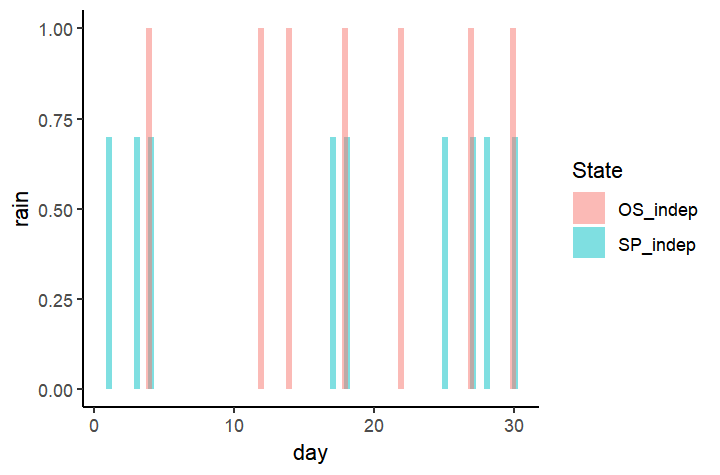
\includegraphics[width=\maxwidth]{figure/rain_graph1-1} 

\end{knitrout}
\footnotesize
$Pr(\text{Rain in Osasco})*Pr(\text{Rain in S\~{a}o Paulo}) = 0.2 * 0.2 = 0.04$ \\
$Pr(\text{Rain in Osasco} \cap  \text{Rain in S\~{a}o Paulo}) = 0.05$ \\
$Pr(\text{Rain in Osasco})*Pr(\text{Rain in S\~{a}o Paulo}) = Pr(\text{Rain in Osasco} \cap  \text{Rain in S\~{a}o Paulo})$ \\
\normalsize

\columnbreak

\begin{knitrout}
\definecolor{shadecolor}{rgb}{0.969, 0.969, 0.969}\color{fgcolor}
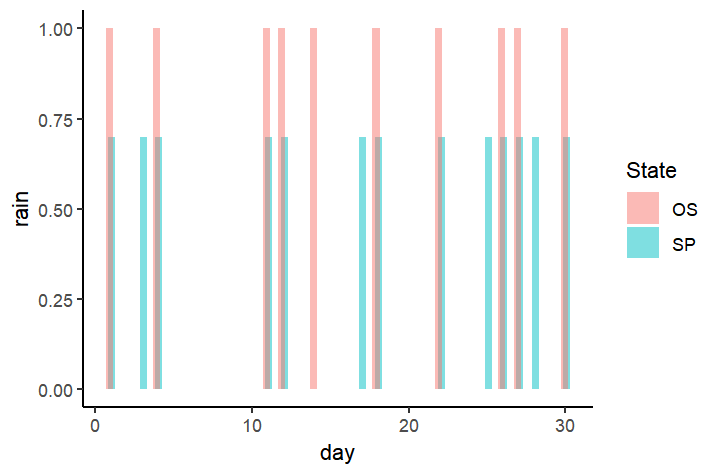
\includegraphics[width=\maxwidth]{figure/rain_graph2-1} 

\end{knitrout}
\footnotesize
$Pr(\text{Rain in Osasco})*Pr(\text{Rain in S\~{a}o Paulo}) = 0.37 * 0.36 = 0.13$ \\
$Pr(\text{Rain in Osasco} \cap  \text{Rain in S\~{a}o Paulo}) = 0.25$ \\
$Pr(\text{Rain in Osasco})*Pr(\text{Rain in S\~{a}o Paulo}) \neq Pr(\text{Rain in Osasco} \cap  \text{Rain in S\~{a}o Paulo})$ \\
\normalsize
\end{multicols}
\end{frame}

\section{Explanation}

\begin{frame}
\frametitle{Explanation}
\begin{itemize}
\item Descriptive Inference
\item Predictive Inference
\item Causal Inference
\end{itemize}
\end{frame}


\begin{frame}
\frametitle{Learning from Data}
\begin{itemize}
\item Why aren't case studies enough?
\pause
\begin{itemize}
\item If we want to know why some countries are more successful democracies than others, surely we have to examine the successful countries in detail?
\pause
\item Yes! But that's not \textit{sufficient}
\pause
\end{itemize}
\item The problem is that there are many variables that \textit{could} explain success
\pause
\item And detailed case studies can help us identify plausible hypotheses
\pause
\item But the only way to \textit{confirm} the hypothesis is to verify that:
\pause
\begin{enumerate}
\item In other cases, the presence of the condition also produces the same outcome (if not, the explanation is not sufficient)
\pause
\item The absence of the condition does not produce the same outcome (if not, the explanation is not necessary)
\end{enumerate}
\end{itemize}
\end{frame}

\begin{frame}
\frametitle{Learning from Data}
\begin{itemize}
\item For example, we could look at India and conclude large Asian countries produce successful democracies
\pause
\begin{itemize}
\item But...China
\pause
\item But...Costa Rica
\pause
\end{itemize}
\item Only by looking at other cases, particularly 'control' cases (small non-Asian countries) can we understand if this explanation is plausible
\end{itemize}
\end{frame}

\begin{frame}
\frametitle{Learning from Data}
\begin{itemize}
\item Even when we compare multiple cases:
\pause
\item \textbf{Correlation is not causation}
\pause
\begin{itemize}
\item If we look hard enough we can always find correlations
\pause
\item By chance...
\pause
\item Due to complex social patterns...
\pause
\item But we cannot conclude that there is a causal effect of $D$ on $Y$
\pause
\end{itemize}
\item \textit{More} data will not help
\pause
\item The problem is the \textit{type} of data; it does not allow us to answer the causal question 
\pause
\item Remember, \textbf{regression only buys you correlation}
\end{itemize}
\end{frame}


% Causal Questions:
% One treatment - causes of effects slide
% One outcome - multiple testing slide

% Later, spend more time on why value valanced POs

\setbeamercolor{background canvas}{bg=}
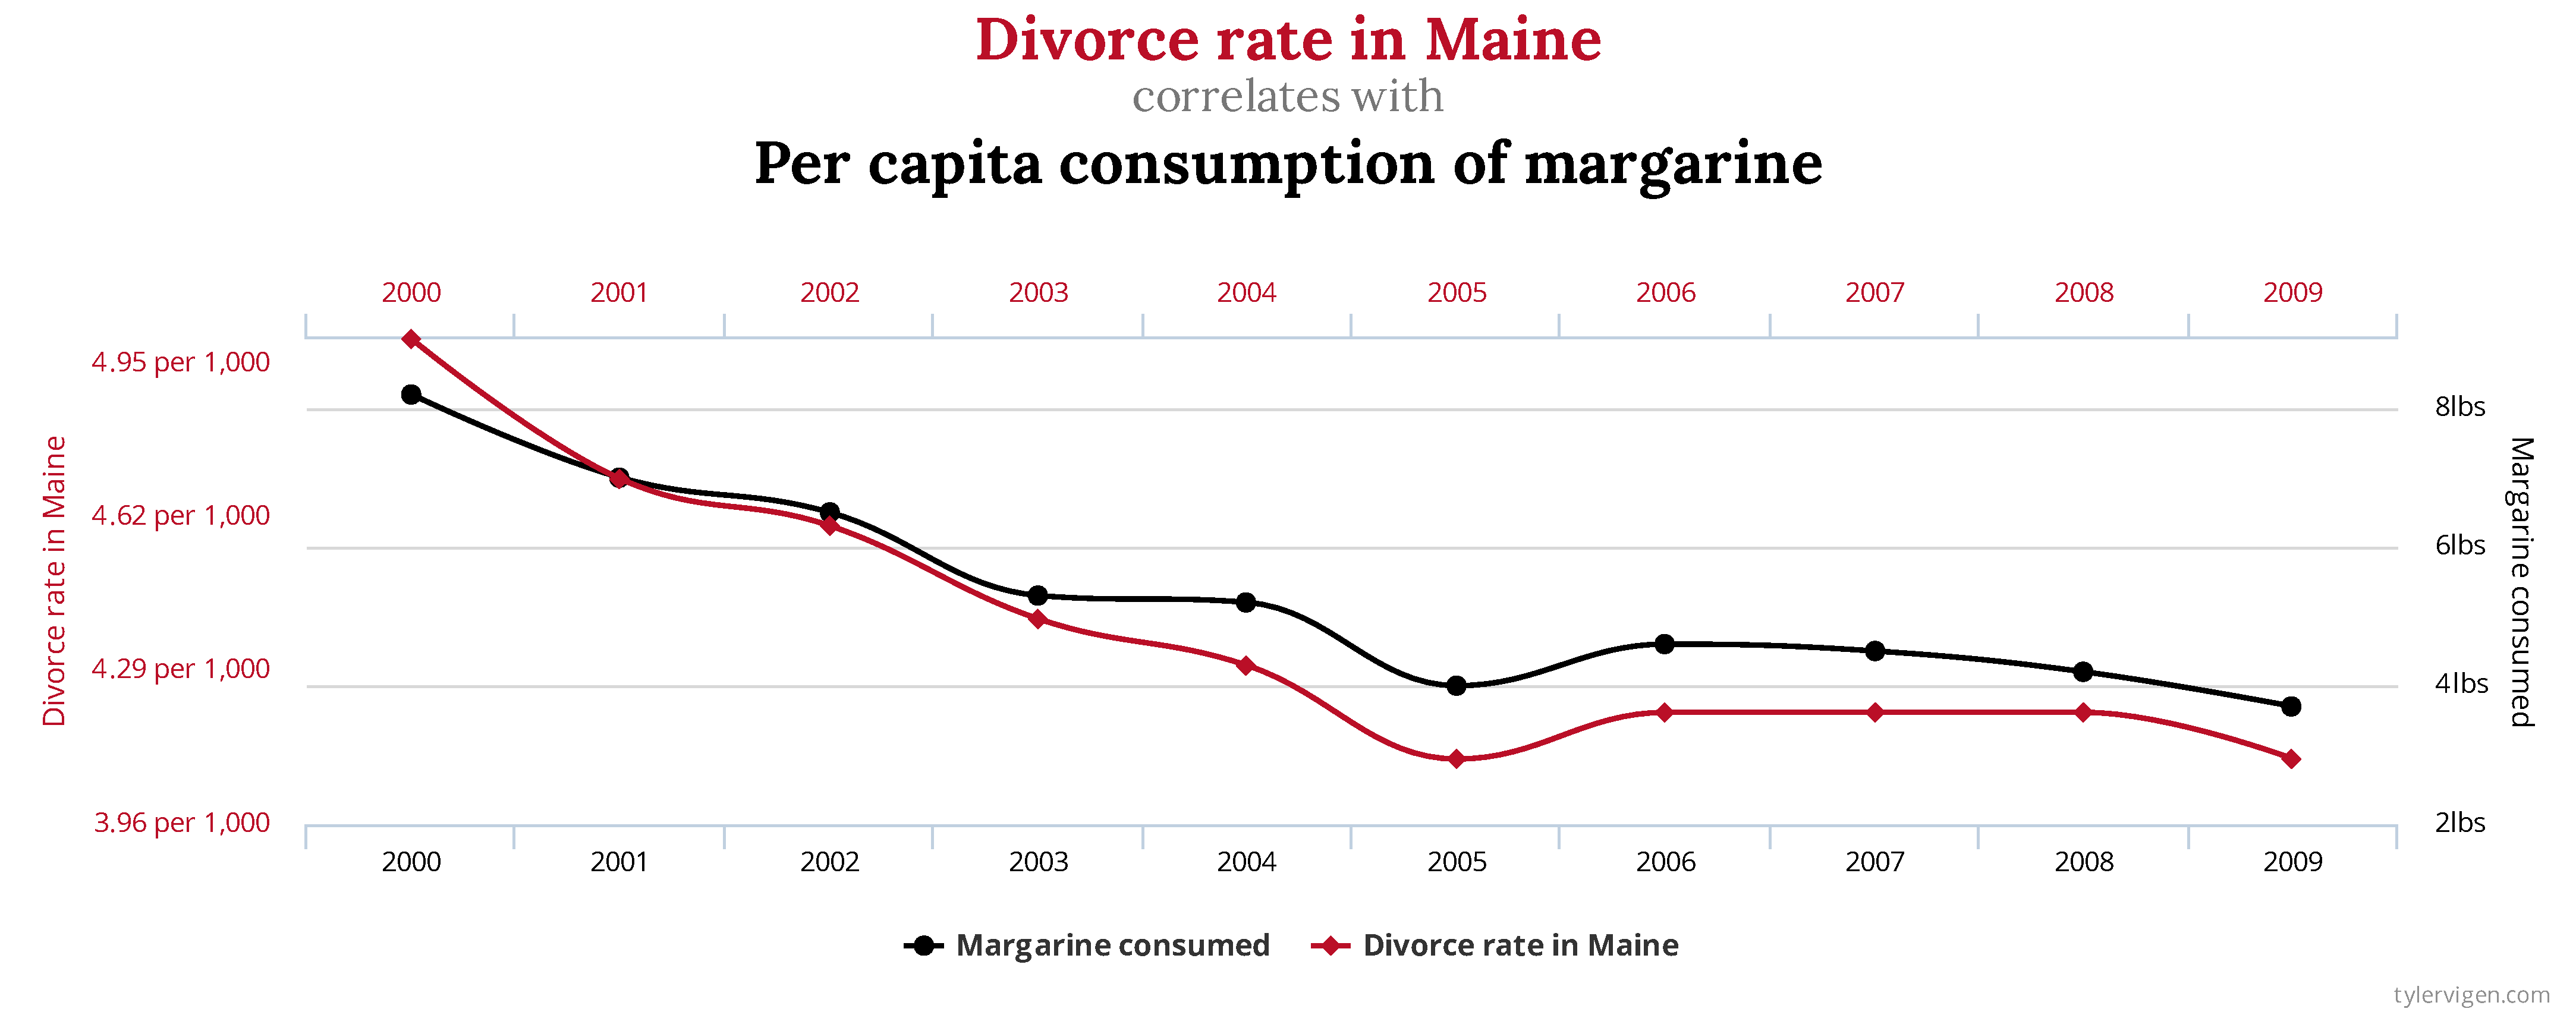
\includepdf[pages={1}]{chart_1.pdf}

\setbeamercolor{background canvas}{bg=}
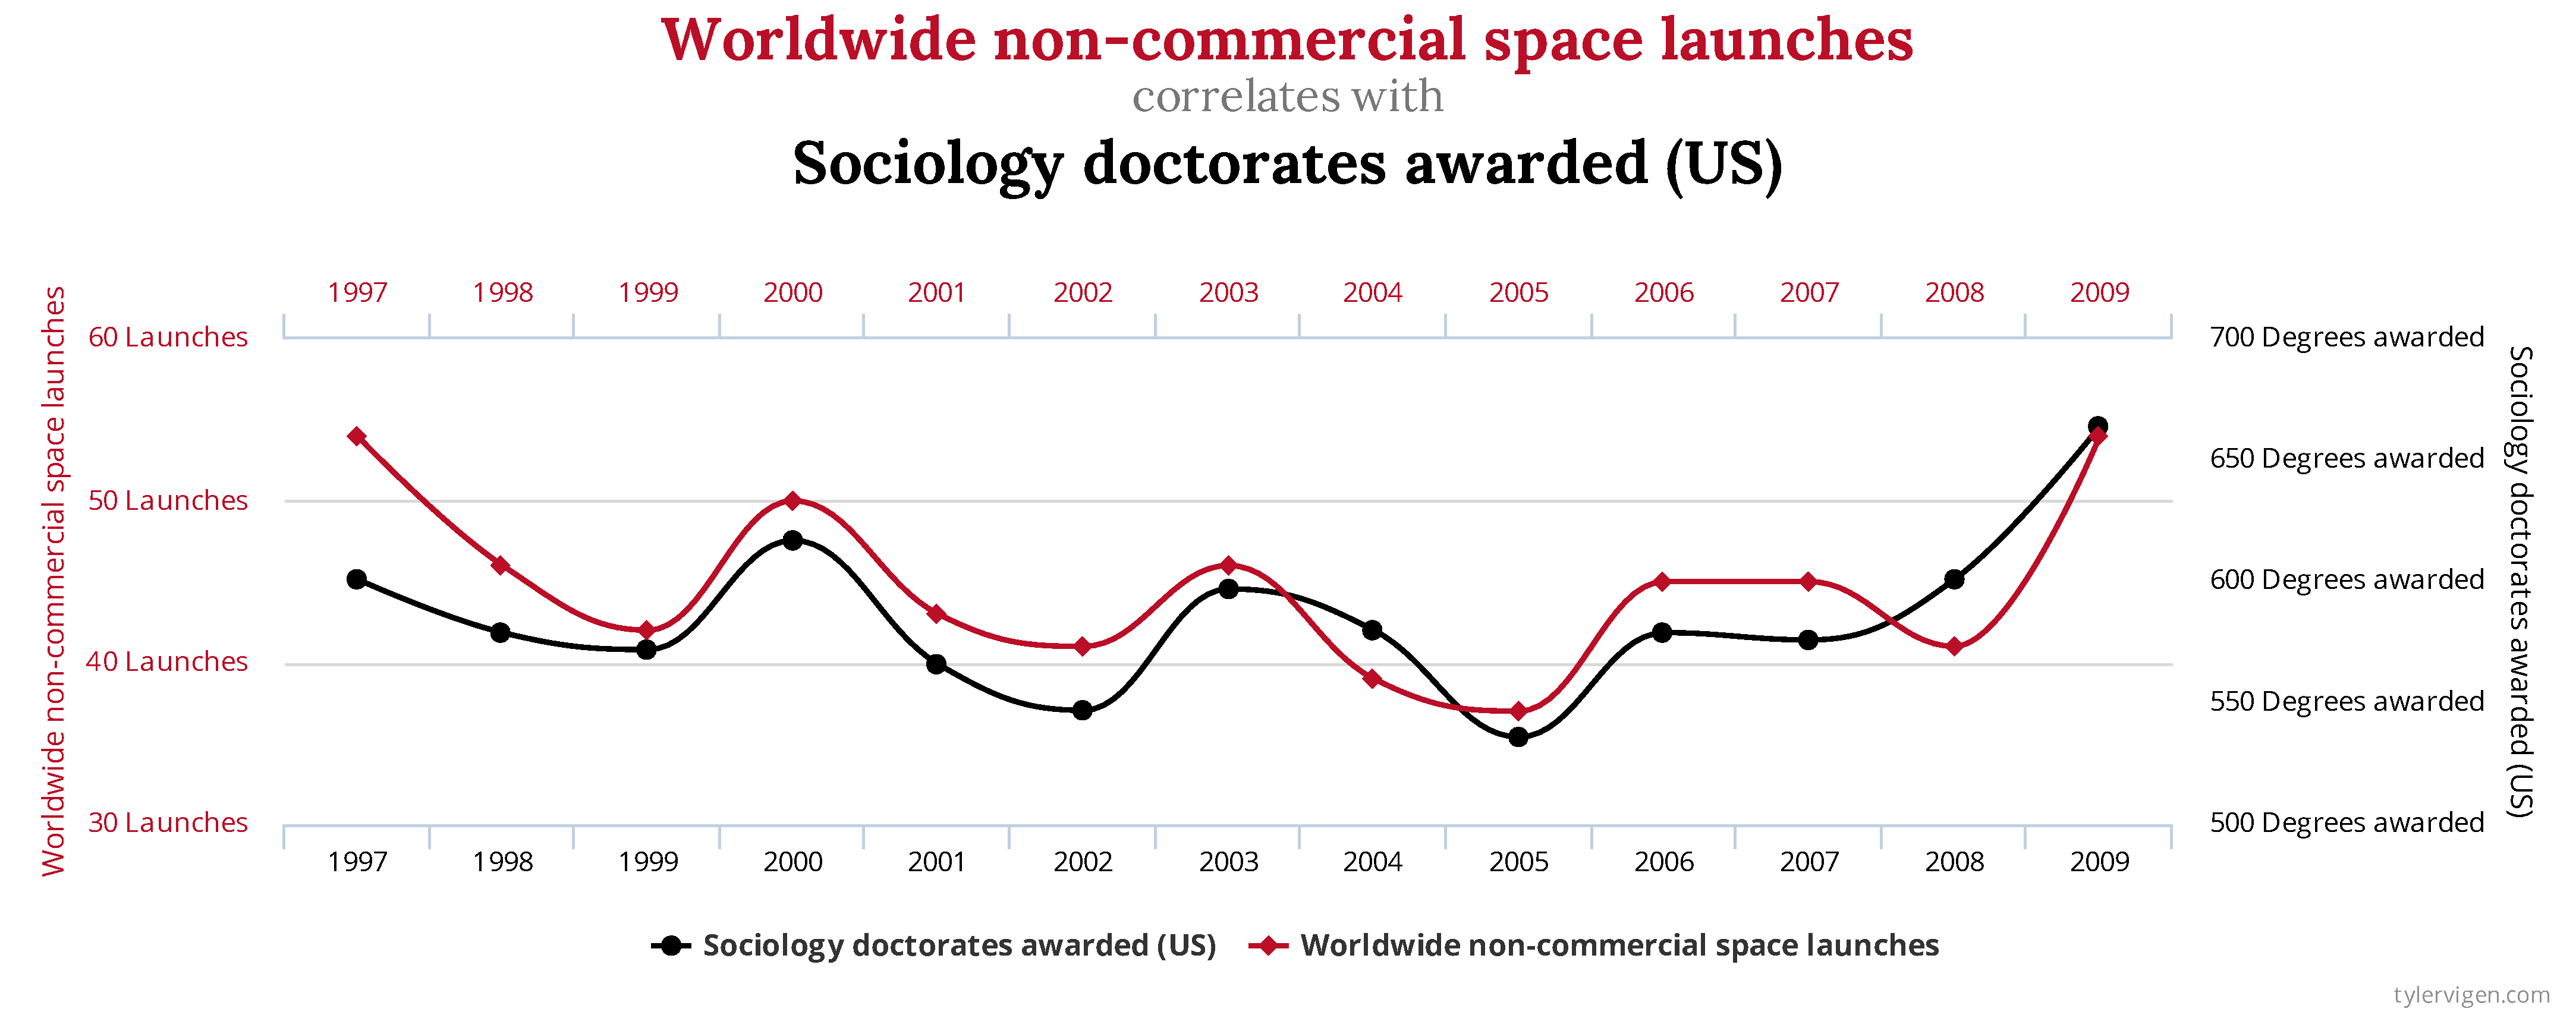
\includepdf[pages={1}]{chart_2.pdf}

\setbeamercolor{background canvas}{bg=}
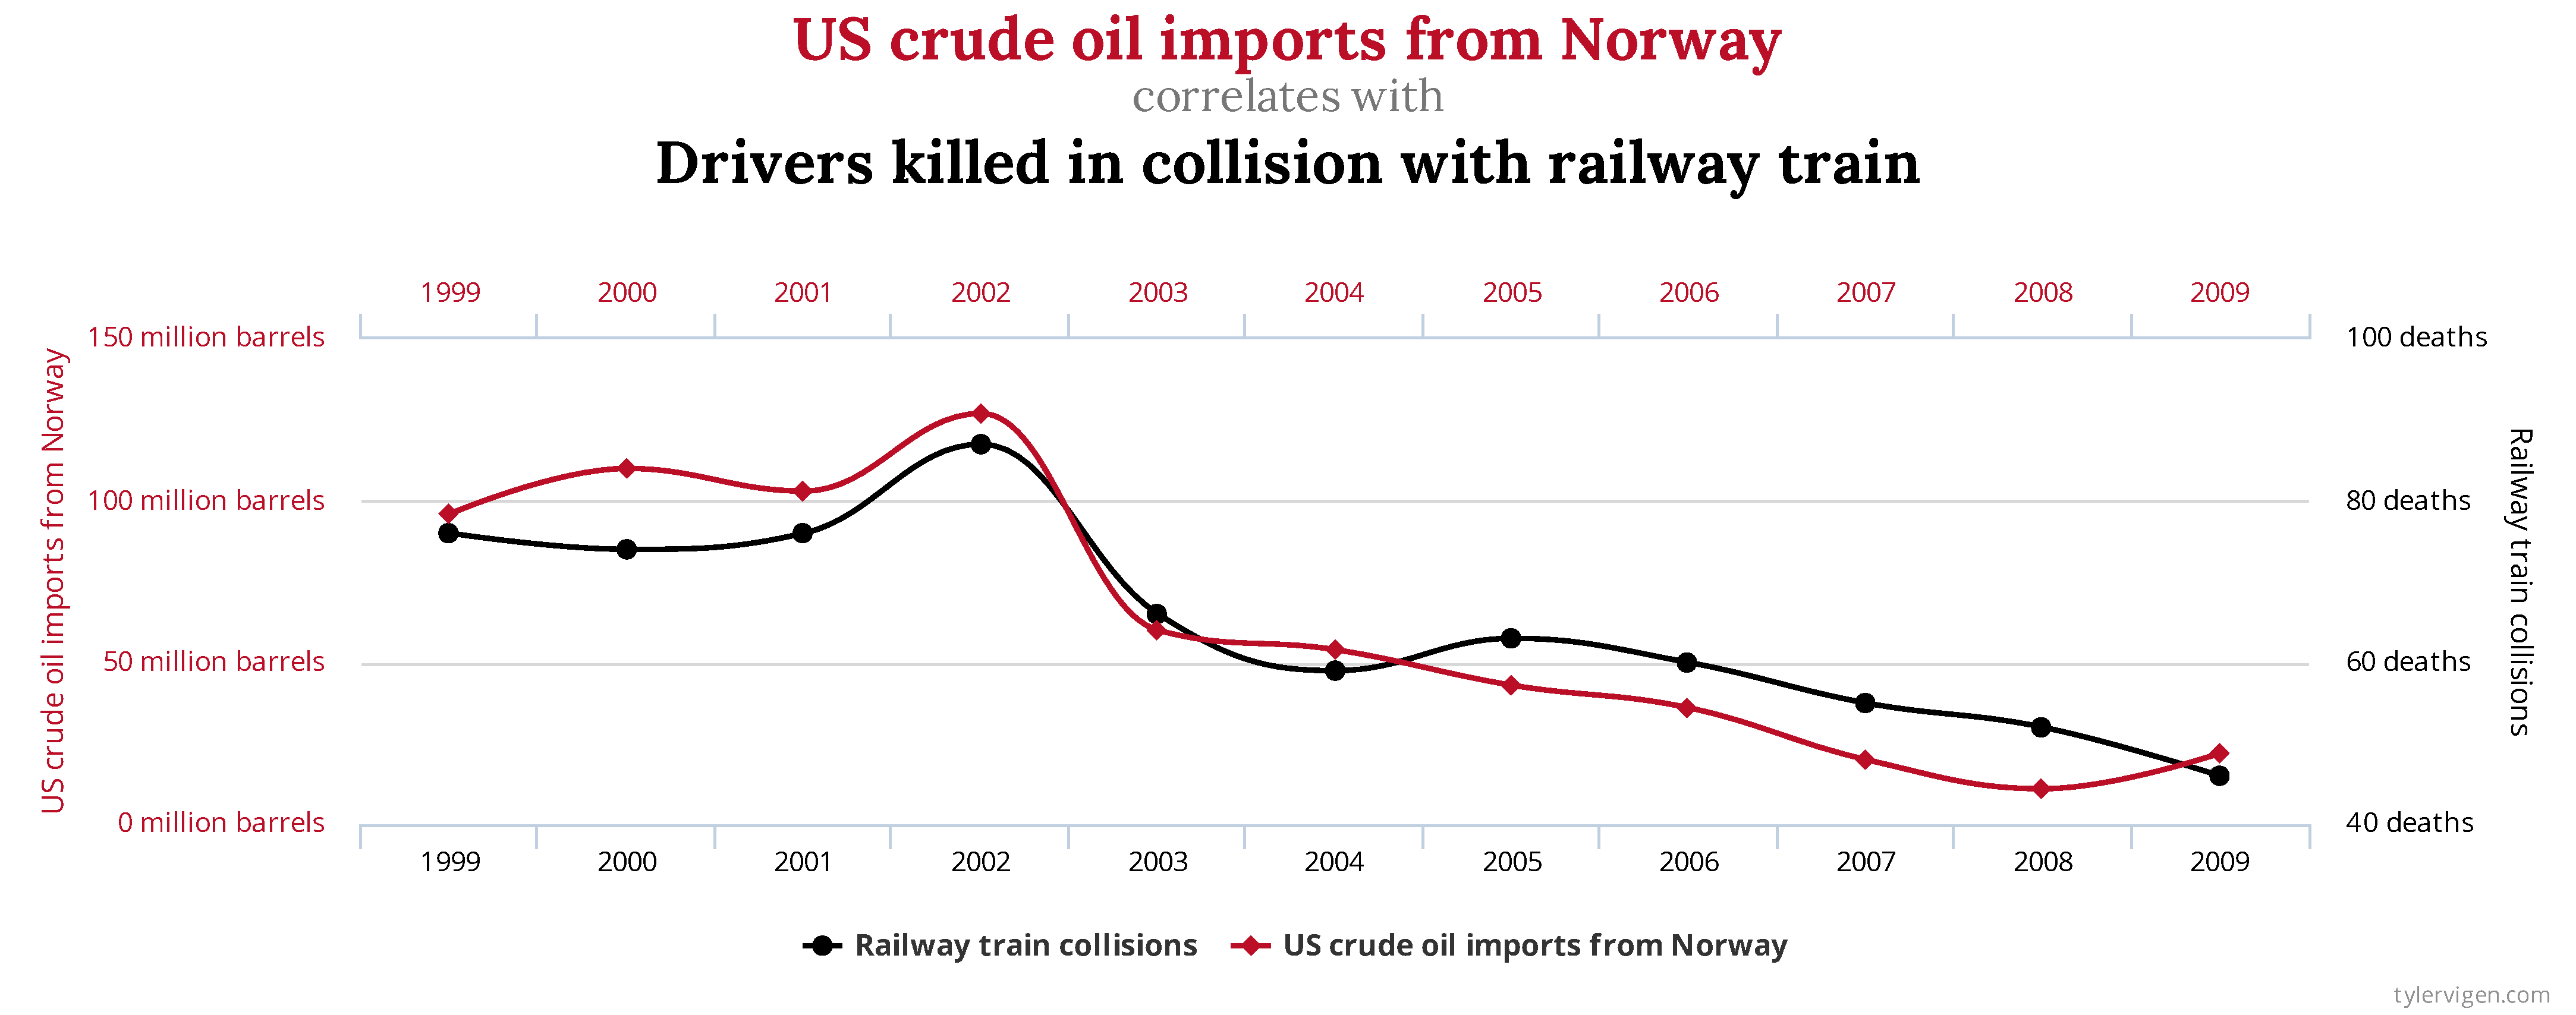
\includepdf[pages={1}]{chart_3.pdf}

\setbeamercolor{background canvas}{bg=}
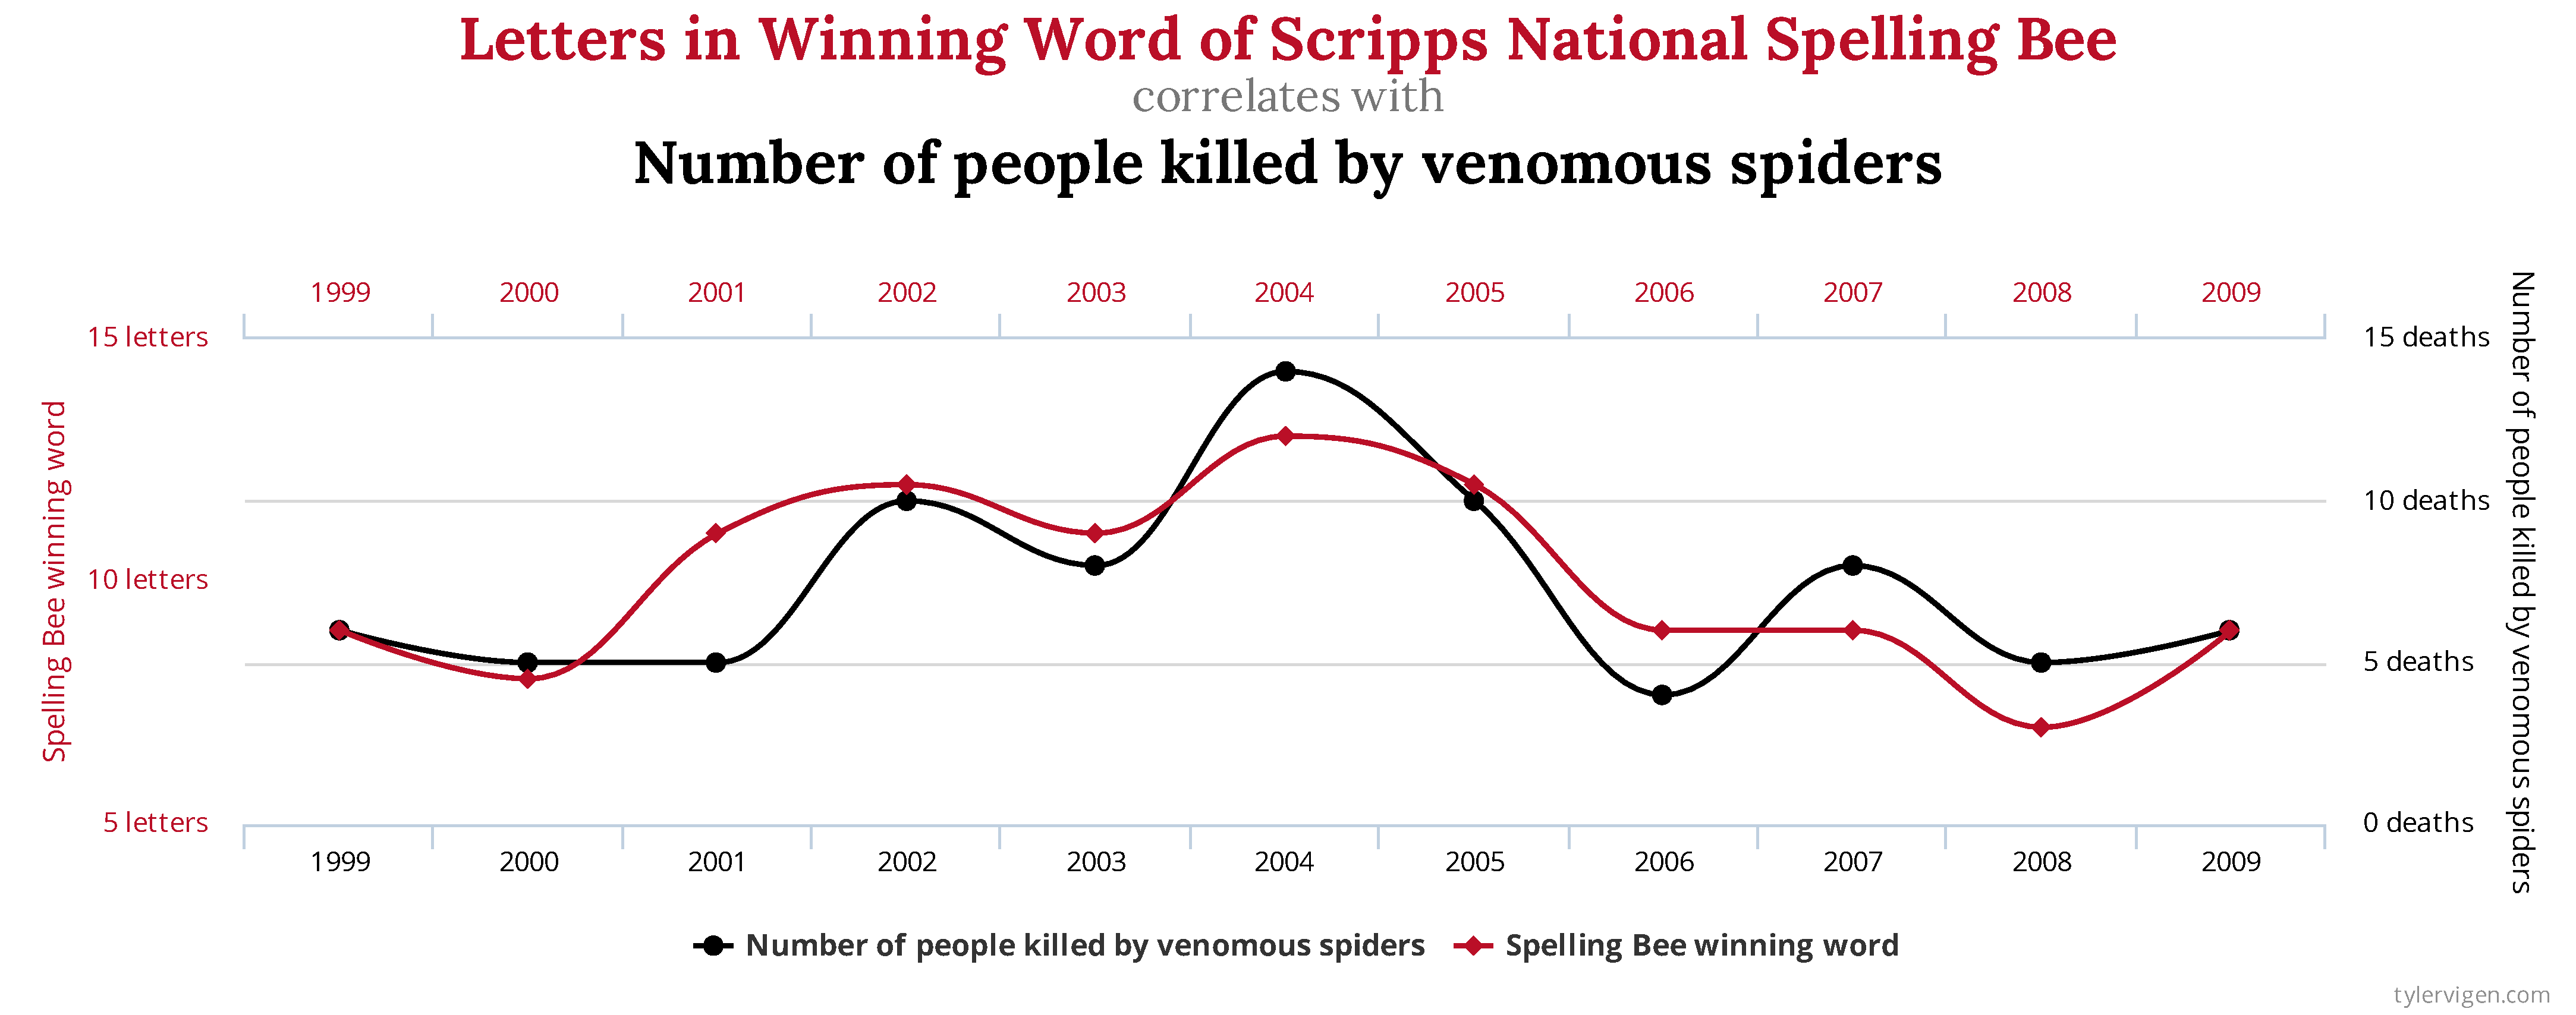
\includepdf[pages={1}]{chart_4.pdf}

\setbeamercolor{background canvas}{bg=}
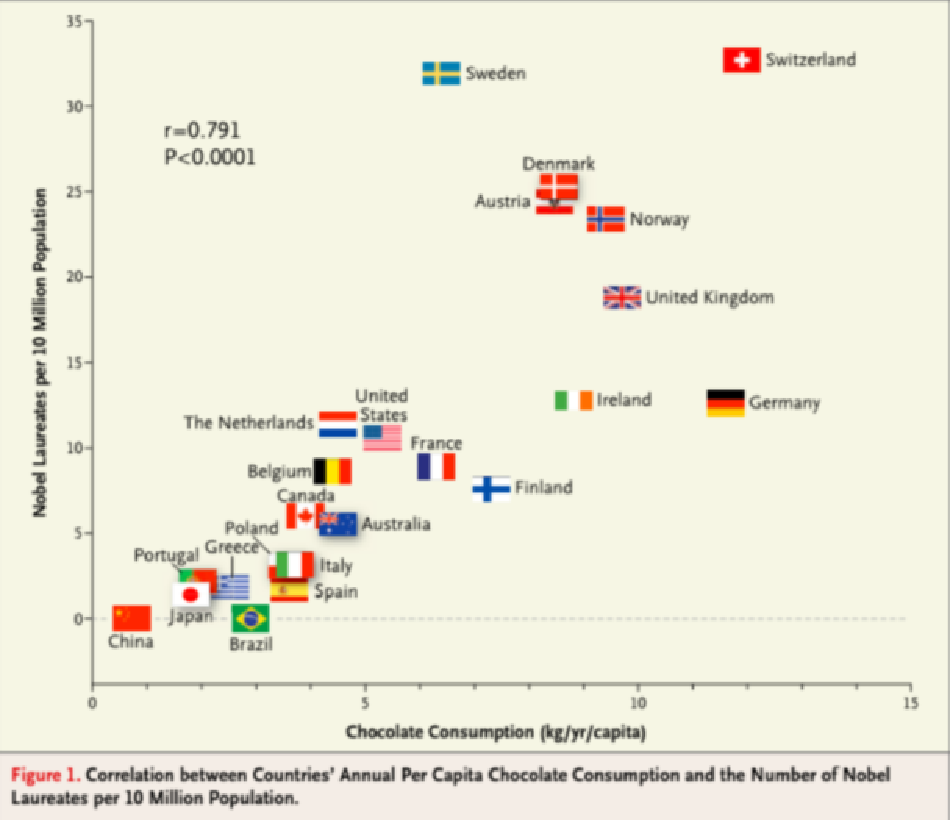
\includepdf[pages={1}]{Chocolate.pdf}

\begin{frame}
\frametitle{Learning from Data}
\begin{itemize}
\item Why isn't correlation enough?
\pause
\begin{itemize}
\item For \textit{prediction}, correlation is fine: If we know a country has chocolate consumption of 10kg/yr/capita we can confidently predict it will have about 25 Nobel Laureates
\pause
\item But for \textit{intervention}, correlation does not help: forcing people to eat more chocolate does nothing on its own to produce more Nobel Laureates
\pause
\end{itemize}
\item So if we want to provide policy-relevant advice, we need to know more than just correlation
\end{itemize}
\end{frame}

\begin{frame}
\frametitle{Learning from Data}
\begin{itemize}
\item Why isn't correlation enough?
\begin{itemize}
\item For \textit{explanation}, correlation also fails - it is no \textit{explanation} to say that Switzerland has the most Nobel Laureates because it has the highest chocolate consumption
\item Explanation means identifying the \textit{direct} and \textit{local} factors that generate Nobel Laureates
\end{itemize}
\end{itemize}
\end{frame}

\begin{frame}
\frametitle{Learning from Data}
\begin{itemize}
\item Why isn't correlation enough?
\pause
\begin{itemize}
\item People are \textbf{strategic}, so their behaviour changes
\pause
\end{itemize}
\item \textbf{The Lucas Critique}: Correlations fall apart when we intervene with policy
\begin{itemize}
\item The data shows no-one lies on their tax forms
\pause
\item So let's abandon tax checks; the government wants to save money
\pause
\item But reducing checks reduces the chances of getting caught
\pause
\item Citizens start to lie on their tax forms
\pause
\end{itemize}
\item That means we need to understand what \textit{causes} people to lie on tax forms, so we can better understand their behaviour
\end{itemize}
\end{frame}

\begin{frame}
\frametitle{Learning from Data}
\begin{itemize}
\item To accumulate knowledge, we have to ask specific types of questions:
\pause
\begin{itemize}
\item Specifically, about the \textbf{effects of causes}
\pause
\end{itemize}
\end{itemize}
\begin{table}[htbp]
  \centering
    \begin{tabular}{|>{\raggedright}p{5cm}|p{5cm}|}
    \toprule
    \textbf{Causes of Effects} & \textbf{Effects of Causes} \\
    \midrule
    What caused Y? & Does X cause Y? \\
    \midrule
    Why did the United States grow faster than Bolivia in the twentieth century? & Did the more permanent colonial settlement of the United States compared to Bolivia affect their subsequent growth rates? \\
    \bottomrule
    \end{tabular}%
  \label{tab:addlabel}%
\end{table}%
\end{frame}


\begin{frame}
\frametitle{Causal Inference}
\begin{itemize}
\item So we need to learn about the \textbf{causal mechanisms} that drive behaviour and shape outcomes
\item The problem is not data \textit{quality}, but how the data were generated
\item We need data generated in ways that reveal the causal mechanism - what would happen if we changed a variable, keeping everything else the same
\end{itemize}
\end{frame}


%Effects of causes


\begin{frame}
\frametitle{Causal Inference}
\begin{itemize}
\item So the type of questions we are asking are NOT "What caused Y?"
\begin{itemize}
\item eg. Why did the United States grow faster than Bolivia in the twentieth century?
\end{itemize}
\item But "Does X affect Y?"
\begin{itemize}
\item eg. Did the more permanent colonial settlement of the United States compared to Bolivia affect their subsequent growth rates? 
\end{itemize}
\item These are called ``Effects of Causes'' questions (not ``Causes of Effects'' questions)
\end{itemize}
\end{frame}

\begin{frame}
\frametitle{Causal Inference}
\begin{itemize}
\item A focus on a single explanatory variable $X$ requires us to clearly define this 'treatment' 
\item AND to clearly define a control
\begin{itemize}
\item What is the opposite of investing \$1bn in education?
\item No investment, or investing it elsewhere?
\end{itemize}
\item Define treatment:
\end{itemize}
\[D_i = 
\begin{cases}
1 \text{, if treated} \\
0 \text{, if not treated}
\end{cases}
\]
\end{frame}

\begin{frame}
\frametitle{Causal Inference}
\begin{itemize}
\item Defining our outcome is also crucial:
\begin{itemize}
\item Can we measure our outcome of interest?
\item Is that outcome the end of the causal chain?
\item Tempting to look at many outcomes, but the risk of cherry-picking
\begin{itemize}
\item All outcomes are probabilistic
\item If we study 20 outcomes, on average one will show a significant effect even with no real causal effect
\end{itemize}
\end{itemize}
\end{itemize}
\end{frame}

\begin{frame}
\frametitle{Causal Inference}
\begin{itemize}
\item Learning about causal effects requires us to specify the `unit' - what is being affected?
\item Countries? Political Parties? Individuals?
\item eg. How does segregation affect attitudes to redistribution?
\begin{itemize}
\item Treatment at the community/societal level
\item Outcome at the individual level
\item Measurement needed at the individual level
\end{itemize}
\item Units are \textbf{time-specific}: the same person 10 minutes later is a different unit
\end{itemize}
\end{frame}

\begin{frame}
\frametitle{Causal Inference}
\begin{itemize}
\item We want to know how some variable affects another variable
\item eg. how a proportional representation electoral system affects investment in education
\begin{itemize}
\item The \textbf{unit} here is any political system where both electoral system and education can vary independently of other units, i.e. countries
\item The \textbf{treatment} is a change to a PR electoral system (vs FPTP)
\item The \textbf{outcome} is the level of (public?) investment in education
\end{itemize}
\end{itemize}
\end{frame}

\section{Causal Inference}

\begin{frame}
\frametitle{Causal Inference}
\begin{itemize}
\item Causality is complex, eg. for $X \rightarrow Y$:
\begin{enumerate}
\item Many factors influence a single outcome ($X1, X2 \rightarrow Y$)
\begin{itemize}
\item Parliamentarism also influences investment in education
\end{itemize}
\item Equifinality: Many routes to the same outcome ($X1+X2 \text{ or } X3+x4 \rightarrow Y$)
\begin{itemize}
\item Ghana and Iceland spend the same on education, but in very different ways
\end{itemize}
\item Reverse causation ($Y \rightarrow X$)
\begin{itemize}
\item A highly educated population might prefer a PR system
\end{itemize}
\item Non-linear impact of one variable on another ($X \Rightarrow Y$)
\begin{itemize}
\item A mixed electoral system may have no effect, but a full PR system might lead to a big jump in investment
\end{itemize}
\item General equilibrium effects - treatment affects many other variables ($X \rightarrow Y1, Y2 \rightarrow Y1$)
\begin{itemize}
\item Public investment in education rises, but private investment falls by the same amount
\end{itemize}
\end{enumerate}
\end{itemize}
\end{frame}

\begin{frame}
\frametitle{Causal Inference}
\begin{enumerate}
\setcounter{enumi}{5}
\item Context matters ($X|Z \rightarrow Y$)
\begin{itemize}
\item PR has a different effect in British vs French legacy education systems
\end{itemize}
\item Treatments cannot be replicated ($X1 \rightarrow Y1, X2 \rightarrow Y2$)
\begin{itemize}
\item Some countries apply open list PR, others closed list etc.
\end{itemize}
\item Spillovers between units ($X_T \rightarrow  X_C \rightarrow Y$)
\begin{itemize}
\item When New Zealand switched to PR, Australia was a natural comparator, but to compete for students, Australia also raised education investment
\end{itemize}
\item Learning, demonstration effects and history matter ($X_{t=1} \rightarrow Y1, X_{t=2} \rightarrow Y2$)
\begin{itemize}
\item New Zealand adopted PR \textit{because} it saw that education improved in Japan
\end{itemize}
\item Social complications eg. emotion, irrationality, chaos theory ($X \rightarrow Y1, X \rightarrow Y2$)
\begin{itemize}
\item New Zealand introduced PR because of an off-hand remark by one person in a campaign 
\end{itemize}
\end{enumerate}
\end{frame}

\begin{frame}
\frametitle{Causal Inference}
\begin{itemize}
\item The \textbf{causal effect} of treatment is how each unit's outcome differs when it is treated and not treated
\pause
\item This means comparing the \textbf{potential outcomes} for unit $i$:
\[
Y_{Di} = 
\begin{cases}
Y_{1i}\text{   Potential Outcome if unit i treated} \\
Y_{0i}\text{   Potential Outcome if unit i not treated}
\end{cases}
\]
\item Treatment Effect $ = Y_{1i} - Y_{0i}$
\end{itemize}
\end{frame}

\begin{frame}
\frametitle{Causal Inference}
\begin{itemize}
\item We are relying on \textbf{counterfactuals}
\pause
\begin{itemize}
\item What would have happened to the same unit if the treatment had not happened?
\pause
\item Would World War I still have happened if Archduke Franz Ferdinand had not been assassinated in 1914?
\pause
\item Would people have voted for Brexit if the campaign had been better regulated? 
\pause
\item Would Brazil have won the 2014 World Cup if Neymar had not been injured?
\pause
\end{itemize}
\item To explain a class of events - not a single event - we need multiple counterfactual comparisons
\end{itemize}
\end{frame}


\begin{frame}
\frametitle{Causal Inference}
\footnotesize
\begin{table}[htbp]
  \centering
  \caption{Potential Outcomes Example}
    \begin{tabular}{|l|p{2.4cm}|p{2.4cm}|r|}
    \hline
          & \multicolumn{1}{p{2.4cm}|}{Investment in Education if PR} & \multicolumn{1}{p{2.4cm}|}{Investment in Education if NOT PR} &  \bigstrut\\
    \hline
          & \multicolumn{1}{l|}{$Y_1$} & \multicolumn{1}{l|}{$Y_0$} & \multicolumn{1}{l|}{Treatment Effect} \bigstrut\\
    \hline
    Brasil & 8     & 4     & 4 \bigstrut\\
    \hline
    Argentina & 10    & 7     & 3 \bigstrut\\
    \hline
    Bolivia & 2     & 4     & -2 \bigstrut\\
    \hline
    Colombia & 11    & 11    & 0 \bigstrut\\
    \hline
    Peru & 6     & 2     & 4 \bigstrut\\
    \hline
    \end{tabular}%
  \label{tab:addlabel}%
\end{table}%
\normalsize
\end{frame}

%Messy - tidy up below
\begin{frame}
\frametitle{Causal Inference}
\begin{itemize}
\item \textbf{The Fundamental Problem of Causal Inference}
\begin{itemize}
\item No units can receive \textbf{both} treatment and control
\item So we can never observe both $Y_1$ and $Y_0$ for the same unit
\end{itemize}
\end{itemize}
\end{frame}

\begin{frame}
\frametitle{Causal Inference}
\footnotesize
\begin{table}[htbp]
  \centering
  \caption{Potential Outcomes Example}
    \begin{tabular}{|p{1.8cm}|p{2.2cm}|p{2.2cm}|p{1.8cm}|r|}
    \hline
          & \multicolumn{1}{p{1.8cm}|}{PR System?} & \multicolumn{1}{p{2.2cm}|}{Investment in Education if PR system} & \multicolumn{1}{p{2.2cm}|}{Investment in Education if FPTP system} &  \bigstrut\\
    \hline
          & \multicolumn{1}{p{1.8cm}|}{$D_i$} & \multicolumn{1}{p{2.2cm}|}{$Y_1$} & \multicolumn{1}{p{2.2cm}|}{$Y_0$} & \multicolumn{1}{p{1.8cm}|}{Treatment Effect} \bigstrut\\
    \hline
    Brasil & 1 & 8     & ?      & ? \bigstrut\\
    \hline
    Argentina & 1 & 10    & ?      & ? \bigstrut\\
    \hline
    Bolivia & 0 & ?     & 4     & ? \bigstrut\\
    \hline
    Colombia & 0 &  ?   & 11    & ? \bigstrut\\
    \hline
    Peru & 0 & ?     & 2     & ? \bigstrut\\
    \hline
    \end{tabular}%
  \label{tab:addlabel}%
\end{table}%
\normalsize
\end{frame}

\begin{frame}
\frametitle{Causal Inference}
\begin{itemize}
\item We can't even look at the change in countries that switch to a PR system
\begin{itemize}
\item What if \textbf{all} countries had started to invest more in education at the same time, for different reasons?
\item The potential outcome for Country X in time 1 is different to at time 2
\end{itemize}
\item So we need to consider the \textbf{counterfactual} - what would have happened if the country had \textbf{not} switched to a PR system?
\item So we can only estimate the effect by comparing \textbf{across} units
\item That is why we are doing causal \textbf{inference}, not causal proof
\end{itemize}
\end{frame}

\begin{frame}
\frametitle{Causal Inference}
\begin{itemize}
\item So we need to consider the exact \textbf{counterfactual} - what would have happened if the country had \textbf{not} switched to a PR system?
\pause
\begin{itemize}
\item This is \textbf{impossible} to know
\pause
\item We can only \textit{estimate} the effect by comparing \textbf{across} units in some way
\pause
\item That is why we are doing causal \textbf{inference}, not causal proof
\end{itemize}
\end{itemize}
\end{frame}

\begin{frame}
\frametitle{Causal Inference}
\begin{itemize}
\item To compare across units we need counterfactuals: \textbf{control} units that do not receive treatment
\item Control units can never be perfect substitutes
\item Causal Inference is all about identifying a \textbf{plausible counterfactual}
\begin{itemize}
\item Plausible means that the potential outcomes of the control unit are the same as those of the treated unit
\end{itemize}
\end{itemize}
\end{frame}

\begin{frame}
\frametitle{Causal Inference}
\begin{itemize}
\item The comparability of treatment and control units depends on how they got to be treated
\begin{itemize}
\item On the \textbf{treatement assignment mechanism}
\end{itemize}
\item If we 'treated' an outlier like B\'{u}zios in Rio, could we find a comparable control unit?
\item Comparisons are easier where the \textbf{treatment assignment mechanism is independent of potential outcomes}
\begin{itemize}
\item This makes it more likely that potential outcomes are 'balanced' and comparable
\end{itemize}
\end{itemize}
\end{frame}

\section{Rest of the Course}

\begin{frame}
\frametitle{Causal Inference}
\begin{itemize}
\item The rest of the course is mostly about the types of treatment assignment mechanisms that \textbf{avoid these biases} and provide plausible counterfactuals
\end{itemize}
\end{frame}

\begin{frame}
\frametitle{Causal Inference}
\begin{enumerate}
\item \textbf{Controlled Experiments} where we \textbf{control} the treatment assignment
\begin{itemize}
\item Field Experiments
\item Survey Experiments
\item Lab Experiments
\end{itemize}
\end{enumerate}
\end{frame}

\begin{frame}
\frametitle{Causal Inference}
\begin{enumerate}
 \setcounter{enumi}{1}
\item \textbf{Natural Experiments} where the assignment mechanism creates balanced potential outcomes
\begin{itemize}
\item Randomized natural experiments
\item Regression Discontinuities
\item Instrumental Variables
\end{itemize}
\end{enumerate}
\end{frame}

\begin{frame}
\frametitle{Causal Inference}
\begin{enumerate}
\setcounter{enumi}{2}
\item \textbf{Observable Studies:} What if no suitable treatment assignments are available?
\begin{itemize}
\item No historical examples of natural experiments
\item Not feasible or ethical to run a field experiment
\end{itemize}
\end{enumerate}
\begin{itemize}
\item Remember the purpose of using these specific treatment assignment mechanisms is to achieve \textbf{comparable potential outcomes}
\item One alternative way of making potential outcomes comparable is to \textbf{selectively use Observable Data}
\begin{itemize}
\item Difference-in-Differences
\item Controlling for confouding variables
\item Matching
\end{itemize}
\end{itemize}
\end{frame}

\begin{frame}
\frametitle{Causal Inference}
\begin{table}[htbp]
  \centering
  \caption{Analysis Types and Assumptions}
    \resizebox*{1.1\textheight}{!}{\begin{tabular}{|r|l|p{2.5cm}|p{2.5cm}|p{2.5cm}|p{6cm}|}
    \hline
    \multicolumn{1}{|r|}{\textbf{Week}} & \multicolumn{1}{l|}{\textbf{Assumption:
}} & \textbf{Researcher Controls Treatment Assignment?} & \textbf{Treatment Assignment Independent of Potential Outcomes} & \textbf{SUTVA} & \multicolumn{1}{p{2cm}|}{\textbf{Additional Assumptions}} \bigstrut\\
    \hline
          & \textbf{Controlled Experiments} &       &       &       &  \bigstrut\\
    \hline
    1     &    Field Experiments & \checkmark & \checkmark & \checkmark &  \bigstrut\\
    \hline
    2     &    Survey and Lab Experiments &  \checkmark & \checkmark & \checkmark & Controlled Environment for treatment exposure \bigstrut\\
    \hline
          & \textbf{Natural Experiments} &       &       &       &  \bigstrut\\
    \hline
    3     &    Randomized Natural Experiments & X     & \checkmark & \checkmark &  \bigstrut\\
    \hline
    4     &    Instrumental Variables & X     & \checkmark & \checkmark & First stage and Exclusion Restriction (Instrument explains treatment but not outcome) \bigstrut\\
    \hline
    5     &    Regression Discontinuity & X     & \checkmark & \checkmark & Continuity of covariates; No manipulation; No compounding discontinuities \bigstrut\\
    \hline
          & \textbf{Observational Studies} &       &       &       &  \bigstrut\\
    \hline
    6     &    Difference-in-Differences & X     & X     & \checkmark & No Time-varying confounders; Parallel Trends \bigstrut\\
    \hline
    7     &    Controlling for Confounding & X     & X     & \checkmark & Blocking all Back-door paths \bigstrut\\
    \hline
    8     &    Matching & X     & X     & \checkmark & Overlap in sample characteristics \bigstrut\\
    \hline
    \end{tabular}}%
\end{table}%
\end{frame}



\begin{frame}
\frametitle{Causal Inference}
\begin{enumerate}
 \setcounter{enumi}{3}
\item \textbf{Small-N studies:} Some research questions have few units available
\end{enumerate}
\begin{itemize}
\item How do we learn about the political economy of development with few units?
\item We can at least avoid some key biases:
\begin{itemize}
\item Comparative Case Studies
\item Process Tracing
\end{itemize}
\end{itemize}
\end{frame}

%treatment assignment mechanism
%potential outcomes
%Y1-Y0 as causal effect but we can't measure/observe. Then introduce counterfactuals/controls only after this.
%We want balance in potential outcomes for controls so plausible counterfactual.
%Treatment assignment influences whether potential outcomes are balanced
%Examples of how certain treatment mechanisms can produce non-balanced potential outcomes and therefore balanced results
%Expectation expressions of how estimate and what real treatment effect is
%Reference to app exploration

%A plausible counterfactual must avoid a number of problems
%Internal validity section here? Sources of bias etc.

\begin{frame}
\frametitle{Causal Inference}
\begin{itemize}
\item But \textbf{how much} can we learn from a causal analysis?
\item Is this an accurate representation of what would happen in the real-world?
\begin{itemize}
\item What was the policy problem (/academic question) you were trying to solve?
\item What details differ? Eg. context of how treatment was applied
\end{itemize}
\item Generalizability to other units (External validity)
\begin{itemize}
\item Would the same thing happen in another country? Next year?
\item Look out for variation in treatment, context, spillovers, learning etc.
\end{itemize}
\item Any generalization requires assumptions
\end{itemize}
\end{frame}

\begin{frame}
\frametitle{Causal Inference}
\begin{itemize}
\item We will try to identify abstract, portable processes
\begin{itemize}
\item \textbf{Causal Mechanisms}
\end{itemize}
\item \textbf{Portable:} If the weather affects election turnout ONLY in Acre, is that a useful causal mechanism?
\item \textbf{Abstract:} If unions are good at mobilizing support, but so are churches, the mechanism is collective action, not union organization
\item We still need to define the \textbf{scope conditions} in which we think this causal mechanism will operate as expected
\end{itemize}
\end{frame}

\begin{frame}
\frametitle{Causal Inference}
\begin{itemize}
\item Examples of Causal Mechanisms:
\begin{itemize}
\item Citizens
\begin{itemize}
\item Electoral Accountability
\item Client Power
\item Collective Action
\item Social Trust/Sanctioning
\item Wealth Effects
\end{itemize}
\item Elites
\begin{itemize}
\item Violence/Coercion
\item Brokerage/Patronage
\item Persuasion/Framing
\item Incumbency Power
\end{itemize}
\item Institutions
\begin{itemize}
\item Power Devolution/Median Voter
\item Network Effects
\item Evolutionary Selection
\item Conversion/Layering/Drift/Replacement
\end{itemize}
\end{itemize}
\end{itemize}
\end{frame}



\begin{frame}
\frametitle{Causal Inference}
\begin{itemize}
\item Examples of Causal Mechanisms:
\begin{itemize}
\item Citizens
\begin{itemize}
\item Electoral Accountability - \textcolor{blue}{Class 5}
\item Client Power - \textcolor{blue}{Class 6}
\item Collective Action - \textcolor{blue}{Class 11}
\item Social Trust/Sanctioning - \textcolor{blue}{Class 4}
\item Wealth Effects
\end{itemize}
\item Elites
\begin{itemize}
\item Violence/Coercion - \textcolor{blue}{Class 8}
\item Brokerage/Patronage - \textcolor{blue}{Class 9}
\item Persuasion/Framing
\item Incumbency Power - \textcolor{blue}{Class 7}
\end{itemize}
\item Institutions
\begin{itemize}
\item Power Devolution/Median Voter - \textcolor{blue}{Class 3}
\item Network Effects
\item Evolutionary Selection
\item Conversion/Layering/Drift/Replacement - \textcolor{blue}{Class 12}
\end{itemize}
\end{itemize}
\end{itemize}
\end{frame}



\end{document}


%setwd('C:\\Users\\Jonny\\Google Drive\\Academic\\USP\\Class\\Week 1 - Intro\\Lecture Slides')
%knitr::knit("Slides_Wk1_intro_5.Rnw")
